\section{Εισαγωγή}
Στόχος αυτού του εργαστηρίου ήταν η μέτρηση των παραμέτρων του συστήματος που δίνεται στο σχήμα~\ref{fig:system}.
\begin{figure}[htb]
    \centering
    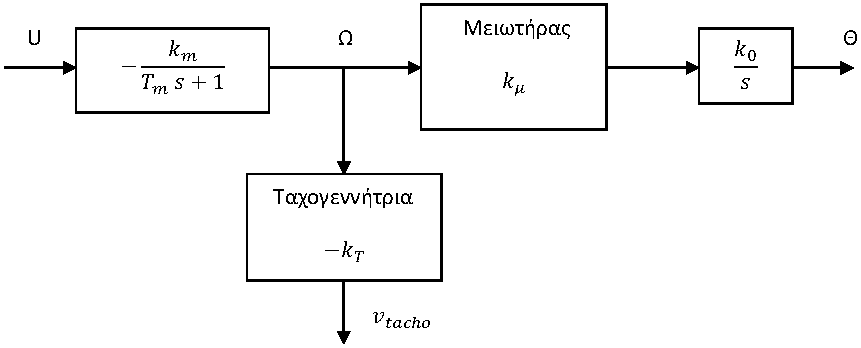
\includegraphics[width=\linewidth]{system}
    \caption[Το δομικό διάγραμμα του συστήματος στο οποίο εργαζόμαστε]%
    {Το δομικό διάγραμμα του συστήματος στο οποίο εργαζόμαστε.
    $U$ είναι η τάση εισόδου, $\Omega$ η ταχύτητα περιστροφής, $\Theta$ η θέση (μέσω τάσης) του άξονα του κινητήρα και $v_{tacho}$ η τάση στη ταχογεννήτρια.}
    \label{fig:system}
\end{figure}
Η λειτουργία του συστήματος και η περιγραφή των ηλεκτρονικών στοιχείων βρίσκεται στην εκφώνηση της άσκησης.

Οι μετρήσεις που παρουσιάζονται στη συνέχεια έγιναν με τα εξής όργανα:
\begin{itemize}
    \item Αριθμός συστήματος: \textbf{Σ8}
    \item Παλμογράφος: \textbf{HM407}
\end{itemize}
